\documentclass{article}
\usepackage{graphicx}
\usepackage[english]{babel}
\usepackage{amsthm}
\usepackage{amssymb}
\usepackage{amsmath}
\usepackage{enumerate} % to be able to use a parametrised enumerate
                       % environment where we can specify how the
                       % items in the environment are labelled.

\newcommand{\nat}{\mathbb{N}}

\title{Homework 6}
\author{CPSC450, Fall2020}
\date{September 30, 2020\\
Due: Tuesday, October 6, 2020}

\begin{document}
\maketitle

\begin{enumerate}

\item For each of the following languages, build a DFA that accepts
  the language.
  \begin{enumerate}
    \item The set of strings of odd length over $\{a, b\}$ that
      contain the substring $bb$.
      \newline 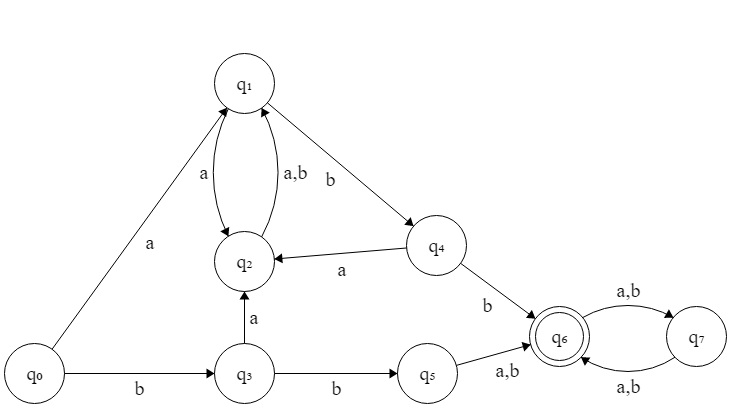
\includegraphics[scale=.5]{hw5#1a.png}

    \item The set of strings over $\{a, b\}$ that contain an even
      number of substrings $ba$.
      \newline 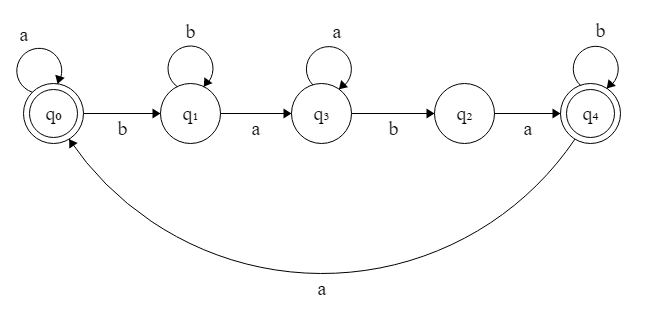
\includegraphics[scale=.5]{hw5#1b.png}
  \end{enumerate}

\item For each of the following languages, build a DFA that accepts
  the language.
  \begin{enumerate}
  \item $\mathbf{(ab)^*ba}$
  \newline 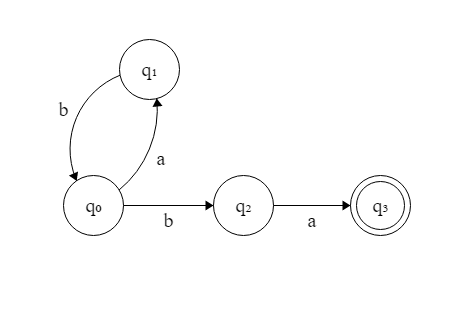
\includegraphics[scale=.5]{hw5#2a.png}
  \item $\mathbf{((aa)^+bb)^*}$
  \newline 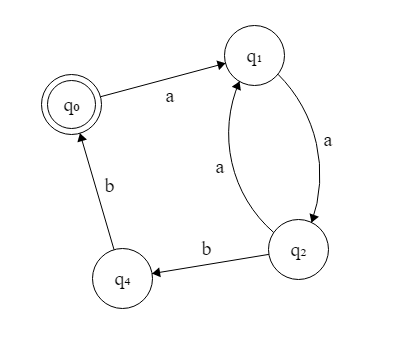
\includegraphics[scale=.5]{hw5#2b.png}
  \end{enumerate}
  
\item For each of the following languages, build an NDFA-$\lambda$
  that accepts the language.
  \begin{enumerate}
    \item The set of strings over $\{a, b\}$ in which each $a$ is
      followed by $b$ or $ab$.
        \newline 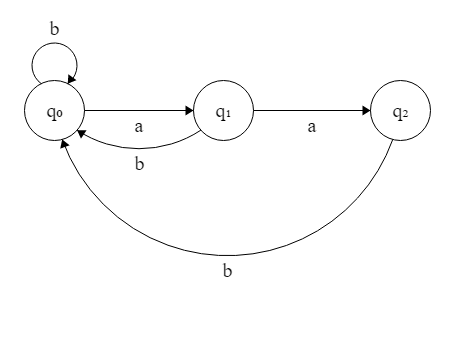
\includegraphics[scale=.5]{hw5#3a.png}
    \item The set of strings over $\Sigma = \{a, b, c\}$ that have a
      substring of length three containing each of the symbols of
      $\Sigma$ exactly once.
      \newline 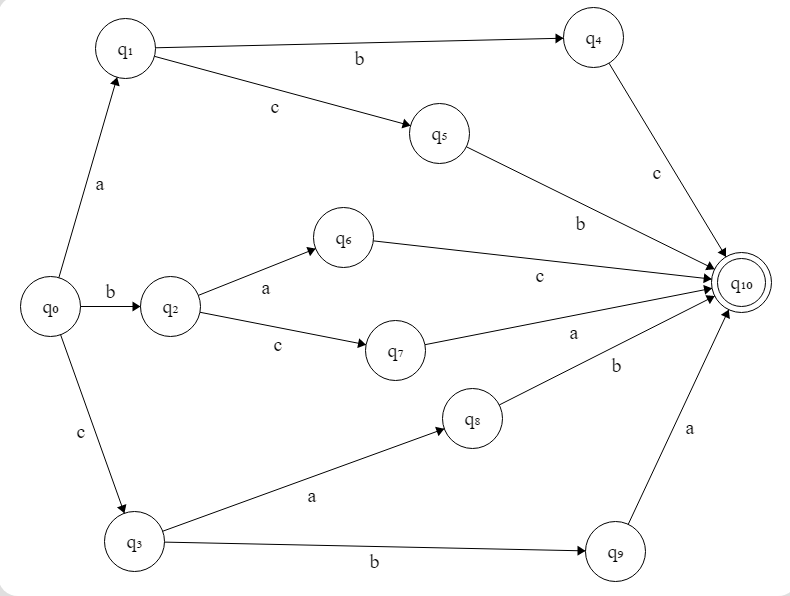
\includegraphics[scale=.5]{hw5#3b.png}

  \end{enumerate}

\end{enumerate}  
     
\end{document}


